\documentclass[12pt]{article}
\usepackage[a4paper, total={7in, 8in}]{geometry}
\usepackage{graphicx,amssymb,dsfont,fourier,xcolor,amsmath,ulem,filecontents,MnSymbol,wasysym}
\usepackage[utf8]{inputenc}

\title{Heat Exchanger Simulation Report: TP1}
\author{User}
\date{29.04.2025}

\begin{document}
\maketitle
\tableofcontents

\section{Introduction}
This report presents the results of the TP1 simulation for a heat exchanger.

\section{Experimental Parameters}
\begin{itemize}
    \setlength\itemsep{-0.5em}
    \item Cold Fluid: water
    \item Hot Fluid: water
    \item Material: stainless steel
    \item Cold Inlet Temperature: 20°C
    \item Hot Inlet Temperature: 40°C
    \item Pipe Length: 2 m
    \item Pipe Diameter: 0.1 m
\end{itemize}\n
\section{Methodology}
The simulation uses the following heat transfer equations:
\begin{equation}\label{eq:tp1_heat_transfer}

    Q = \dot{m} \cdot c_p \cdot (T_{out} - T_{in}) \quad \text{(Heat transfer)} \\
    Q = U \cdot A \cdot \Delta T_{lm} \quad \text{(Overall heat transfer)}
    
\end{equation}\n
\section{Results and Discussion}
\begin{figure}[htb!]
        \centering
        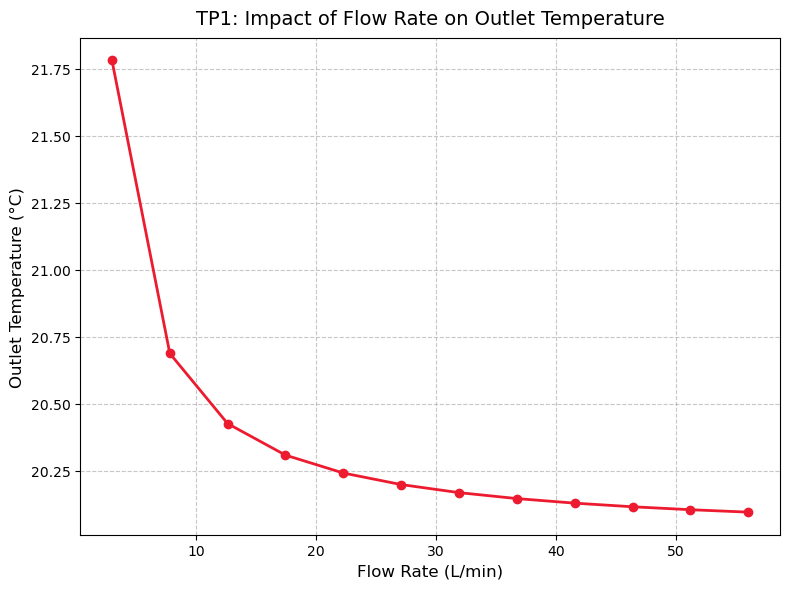
\includegraphics[width=0.8\textwidth]{tp1_plot.png}
        \caption{Simulation results for TP1}
        \label{fig:tp1_results}
\end{figure}\n\begin{table}[ht!]
        \centering
        \begin{tabular}{|l|c|c|c|}
\hline
Flow Rate (L/min) & Outlet Temp (°C) & Heat Transferred (W) & Efficiency (%) \\
\hline
5.0 & 22.42 & 844.17 & 12.1 \\
\hline
15.555555555555555 & 20.82 & 885.73 & 4.08 \\
\hline
26.11111111111111 & 20.49 & 894.03 & 2.45 \\
\hline
36.666666666666664 & 20.35 & 897.59 & 1.75 \\
\hline
47.22222222222222 & 20.27 & 899.56 & 1.37 \\
\hline
57.77777777777778 & 20.22 & 900.82 & 1.12 \\
\hline
68.33333333333333 & 20.19 & 901.69 & 0.95 \\
\hline
78.88888888888889 & 20.16 & 902.33 & 0.82 \\
\hline
89.44444444444444 & 20.14 & 902.81 & 0.72 \\
\hline
100.0 & 20.13 & 903.2 & 0.65 \\
\hline
\end{tabular}
        \caption{Results for TP1: Flow Impact}
        \label{tab:tp1_results}
\end{table}\n
\section{Conclusion}
The simulation results show the impact of the varied parameter on the outlet temperature, heat transferred, and efficiency.

\end{document}
